\chapter{Establishing a Baseline Performance}

\epigraph{\itshape Success is built sequentially. It's one thing at a time.}{---Gary W. Keller}

The objective of this thesis is to enhance the classification of underwater acoustic signals by refining preprocessing techniques and feature extraction methods. As with any scientific endeavour, it is essential to first establish a benchmark -- a reference point that serves as the foundation for measuring progress. This chapter lays out the baseline classifier architecture that will be used consistently throughout all subsequent experiments. By keeping the classifier architecture constant, we ensure that any performance improvements are solely attributed to changes in the preprocessing or feature extraction methods, rather than from adjustments in the classifier.

This chapter is organised as follows. We begin by introducing the dataset, detailing the process of segmenting it into folds to enable cross-validation during training. We also examine the class distribution across the dataset and within each fold, identifying any imbalances that may influence model performance.

Next, we describe the chosen classifier architecture -- a hybrid \acrshort{cnnlstm} model that combines the spatial feature extraction capabilities of convolutional layers with the temporal pattern recognition strengths of \acrshort{lstm} layers. This model will serve as the foundation for all further experiments in this thesis. We discuss the feature inputs for the model, specifically the power spectrograms derived from each audio sample, and outline the process of extracting these using MATLAB, including key parameters such as the \acrshort{fft}, window size, overlap percentage, and frequency resolution. 

Lastly, we cover the approach to hyperparameter tuning to maximise the model's baseline performance. We conclude with a discussion of the coding frameworks and libraries used, as well as the hardware setup, including the GPU utilised for training. This ensures a comprehensive understanding of the baseline model's development, configuration, and evaluation.

%%%%%%%%%%%%%%%%%%%%%%%%%%%%%%%%%%%%%%%
\section{The dataset: DeepShip}

The dataset selected for this study is the DeepShip dataset \cite{irfan_deepship_2021}. There are two key reasons behind this choice. Firstly, DeepShip has become the authoritative benchmark dataset for \acrshort{uatr}, with many recent scientific studies reporting their performance metrics on this dataset. Given its extensive use, the dataset provides a solid foundation for evaluating new techniques, allowing direct comparison with a vast body of prior work. Additionally, past research students at Thales have also worked with DeepShip, publishing their findings, which provides continuity for our work and the opportunity to build upon their results.

Secondly, while the newly released OceanShip dataset (see Section \ref{subsubsec:oceanship}) offers more recordings -- over twice the length of DeepShip -- it is currently inaccessible due to issues with the international accessibility of the cloud storage provider chosen by its authors. More importantly, the class labels within OceanShip have not been externally validated, raising concerns over the quality and reliability of its data. In contrast, DeepShip has undergone independent verification by sonar processors at Thales, ensuring its labels are accurate and reliable for research purposes.

\subsection{Dataset overview}

As outlined in Section \ref{subsubsec:deepship}, the DeepShip dataset consists of 613 recordings from 265 ships, categorised into four vessel classes (see Table \ref{tab:deepship-summary} for more information). However, some of the recordings in the original dataset lacked metadata, leading us to work with a refined subset of DeepShip for this thesis. This subset includes 582 of the 613 recordings, representing 249 of the 265 vessels. Consequently, the dataset length is slightly reduced to 2684 minutes, compared to the original 2824 minutes. Table \ref{tab:deepship-subset} compares the number of ships, recordings, and total recording time for each vessel class in our subset (values outside parentheses) with the original dataset (values inside parentheses). Hereafter, this subset will be referred to simply as DeepShip.

Like many real-world datasets, DeepShip exhibits minor class imbalance, with some ship classes being more heavily represented than others. A class distribution analysis was conducted to visualise this imbalance. Figure \ref{fig:deepship-subset-recording-length} illustrates the variation in the duration of recordings for a vessel. As shown, there is at least one outlier vessel in each class that is significantly over-represented. For example, the median recording duration of all cargo vessels is 5.9 minutes, yet the cargo vessel \texttt{PRINCESS\_SUPERIOR} has over 151 minutes of sonar signal data. Also, the number of ships and number of recordings in each class is quite unbalanced (Figure \ref{fig:deepship-subset-number-vessels}), however the overall total recording time of each class is fairly balanced (Table \ref{tab:deepship-subset}).

\begin{table}[tb]
\centering
\begin{tabular}{llll}
\toprule
\textbf{Vessel class} & \textbf{Ships} & \textbf{Recordings} & \textbf{Total recording time (min)} \\ \midrule
Cargo & 62 (69) & 106 (110) & 628 (640) \\
Passengership & 43 (46) & 180 (193) & 715 (742) \\
Tanker & 128 (133) & 234 (240) & 735 (765) \\
Tug & 16 (17) & 62 (70) & 606 (677) \\
\textbf{Total} & \textbf{249 (265)} & \textbf{582 (613)} & \textbf{2684 (2824)} \\ \bottomrule
\end{tabular}
\caption{Comparison of the DeepShip subset used in this thesis (values outside parentheses) with the complete DeepShip dataset (values in parentheses).}
\label{tab:deepship-subset}
\end{table}

\begin{figure}[p]
    \centering
    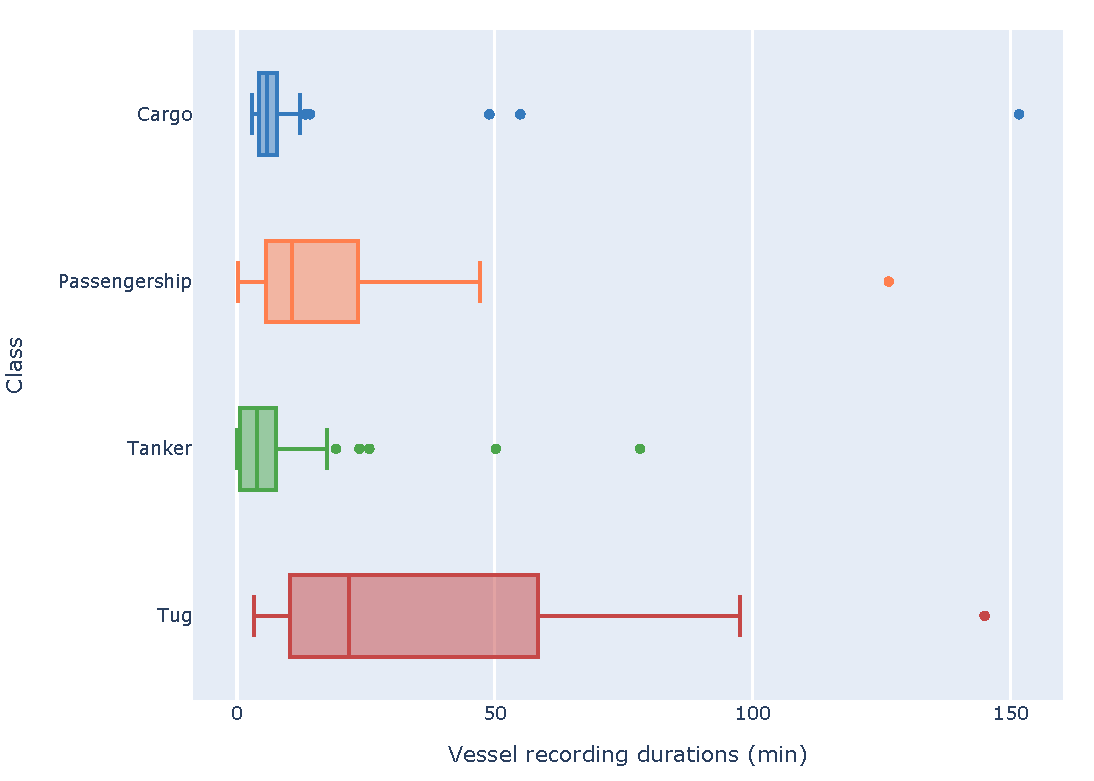
\includegraphics[width=0.9\textwidth]{img/ch3/deepship_duration_spread.pdf}
    \caption{The distribution of vessel recording durations in our DeepShip subset, split by class.}
    \label{fig:deepship-subset-recording-length}
\end{figure}

\begin{figure}[p]
    \centering
    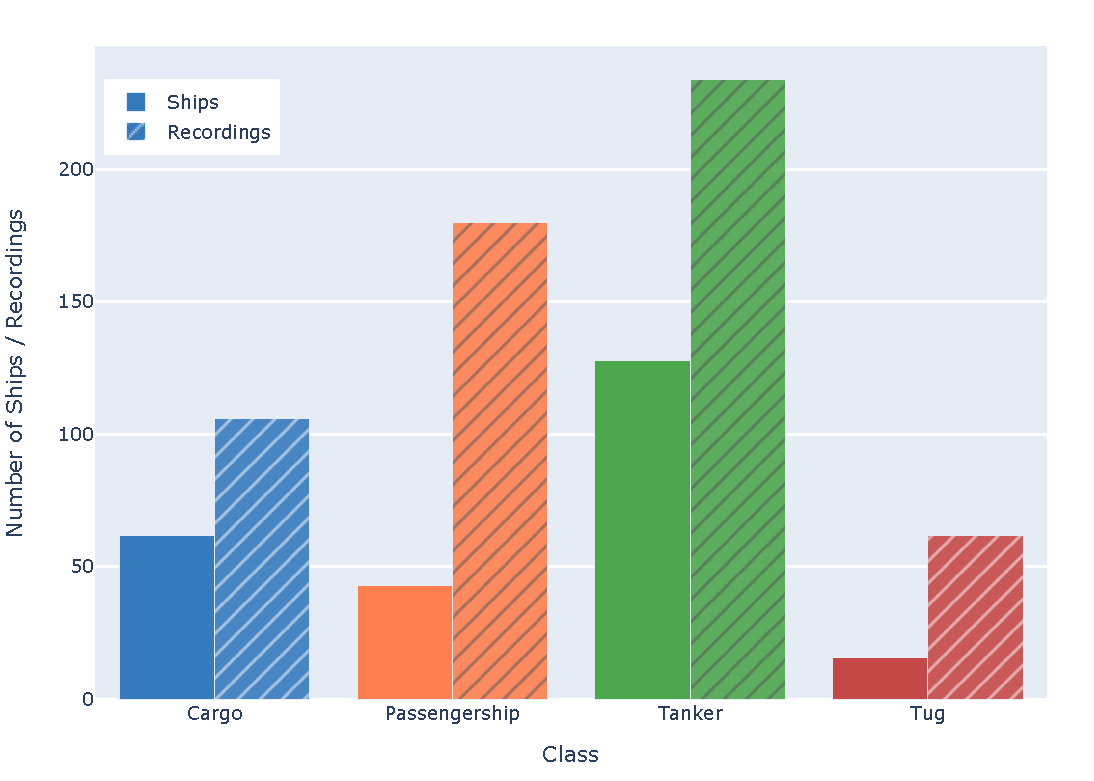
\includegraphics[width=0.9\textwidth]{img/ch3/deepship_class_analysis.pdf}
    \caption{The number of vessels and number of recordings in each class of the DeepShip subset, split by class.}
    \label{fig:deepship-subset-number-vessels}
\end{figure}

\subsection{3-second segmentation}

A widely used approach in audio applications for machine learning is to split each audio recording into smaller segments to boost the number of training samples, improve granularity in feature extraction, and allow more robust classification models to be trained. Segmenting the data into smaller clips enables better generalisation by providing the model with more diverse examples and variations across the data. Additionally, smaller, more homogeneous segments can allow the model to focus on the most relevant features while ignoring background noise components, thereby improving classification performance \cite{xu_self-supervised_2023}. Some examples of \acrshort{uatr} literature which employ segmentation on the DeepShip dataset include: Li et al. \cite{li_underwater_2022}, who segmented the DeepShip dataset into 5-second clips to yield 11,174 samples, using a 70-20-10 split for training, verification, and test datasets respectively; Chen et al. \cite{chen_hierarchical_2024}, who segmented DeepShip into 5-second segments and then divided each class into five equal folds at random; and Sun and Leo \cite{sun_underwater_2023}, who used a 3-second segmentation strategy for DeepShip, acknowledging the importance of segmenting audio to increase the number of samples and make the dataset more computationally feasible for machine learning models. 

The choice of 3-second segments, specifically, is also grounded in previous studies, which have demonstrated that this interval strikes an optimal balance between maintaining sufficient audio context for accurate classification and also managing the model's computational complexity. Longer segments may provide more stability and context, however they also increase computational demands and the risk of overfitting by capturing more irrelevant or noisy information \cite{chen_ship-radiated_2024, li_underwater_2022}. Conversely, shorter segments may lack sufficient context, with burst noise or transient phenomena in the signal having a more pronounced negative impact on classification accuracy \cite{shen_auditory_2018, tang_deep_2024}. Thus, the 3-second segment length aims to achieve an effective balance between data complexity and computational efficiency. This segment length is consistent with other state-of-the-art studies that similarly found 3-second segments optimal for underwater acoustic target recognition tasks \cite{xu_self-supervised_2024, tang_deep_2024}. Notably, the original authors of the DeepShip dataset also chose to divide each recording into 3-second segments, further validating this selection \cite{irfan_deepship_2021}.

In total, DeepShip, with a total recording time of 2684 minutes (161,040 seconds), was segmented into 53,680 3-second segments. After removing segments containing only background noise or silence -- to ensure that the inputs were actually representative of ship noise patterns -- there were a total of 53,503 valid segments remaining.

\subsection{Distribution of segments into folds}

In auditory applications of machine learning, it is common practice to divide input audio clips into $k$ folds for cross-validation \cite{chi_classifying_2022, basili_classification_2004, zeng_spectrogram_2019, chen_ship-radiated_2024, chen_hierarchical_2024}. The most common approach is \textit{leave-$p$-out cross-validation}, where $p$ folds are used for training and the remaining $k-p$ folds for testing. This process is repeated until each fold has been used for both training and testing. In cases where the dataset allows, \textit{stratified $k$-fold cross-validation} is preferred, as it ensures that each fold contains an equal number of samples from each class. However, this ideal design is not always feasible due to the original dataset's class distribution.

Hence, following best practice, after segmentation the dataset was divided into 10 folds with an effort to maintain an approximately equal number of 3-second segments from all four ship classes in each fold. A Python script was used to automate this process, generating a CSV file that specifies the assignment of each 3-second segment to a fold.

Two key considerations guided the design of the 10-fold split for DeepShip. First, to prevent the model from learning recording-specific characteristics, such as background noise or vessel-specific nuances, all clips derived from a given recording were placed in the same fold \cite{chi_classifying_2022}. Second, given that \acrshort{uatr} datasets often contain multiple recordings from the same vessels, we aimed to distribute an approximately equal number of samples from each vessel across the folds. This not only helps balance the class distribution within each fold but also ensures that each vessel is consistently represented across the folds, improving the robustness of the model evaluation.

It should be noted, however, that the split is not perfectly uniform; some variability exists in the number of segments per fold. For instance, the Tug class exhibits the largest variation, with Fold 1 containing only 360 segments, while Fold 3 contains 3006. The complete distribution of samples across the 10 folds is shown in Figure \ref{fig:10-fold-overview}. 

This variability arises from the constraints mentioned above: entire recordings, rather than individual segments, were assigned to each fold to avoid splitting a recording across multiple folds. Furthermore, efforts to distribute an equal number of samples from each vessel across the folds were limited by the inherent imbalance in recording durations within the DeepShip dataset (Figure \ref{fig:deepship-subset-recording-length}). Despite the resulting variability, this method still enhances the dataset's integrity by ensuring that no recording is split across multiple folds, ultimately improving the consistency and robustness of the dataset for cross-validation.

\begin{figure}[htbp]
    \centering
    % Subfigure 1: Fold counts by class
    \begin{subfigure}[t]{\textwidth}
        \centering
        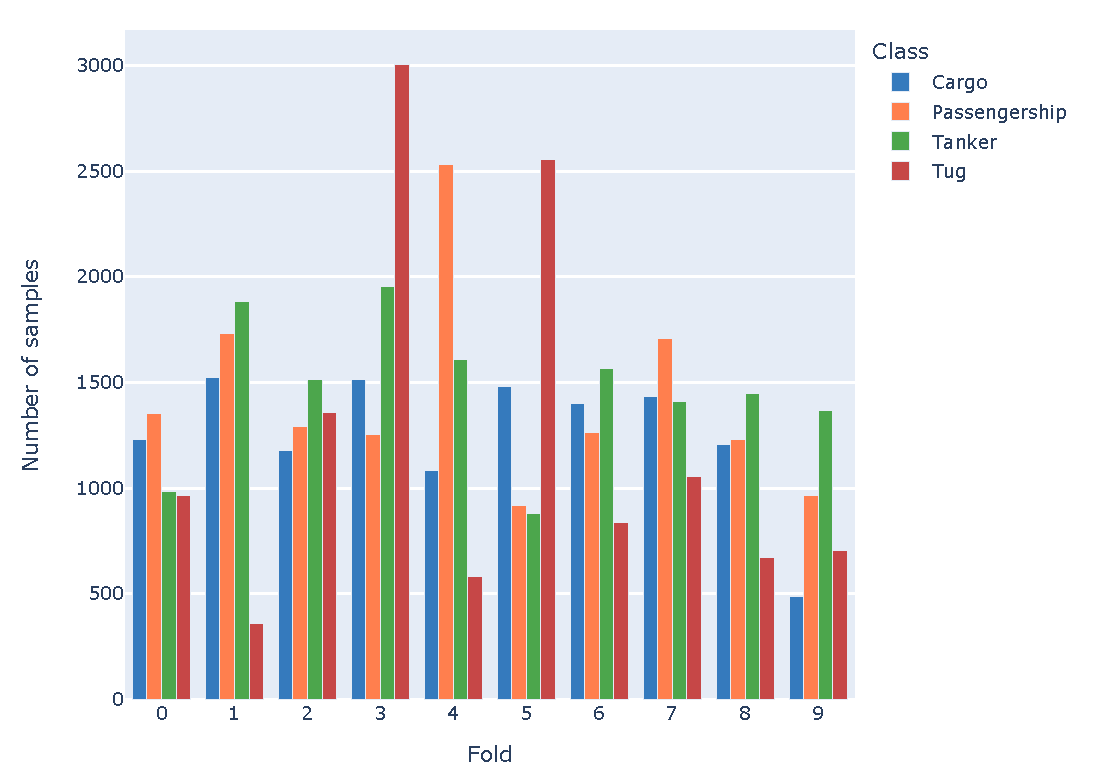
\includegraphics[width=0.95\textwidth]{img/ch3/10_folds_counts.pdf}
        \caption{Count of samples in each fold by class}
        \label{fig:10-fold-counts}
    \end{subfigure}
    
    % Subfigure 2: Sample counts by fold 
    \begin{subfigure}[t]{\textwidth}
        \centering
        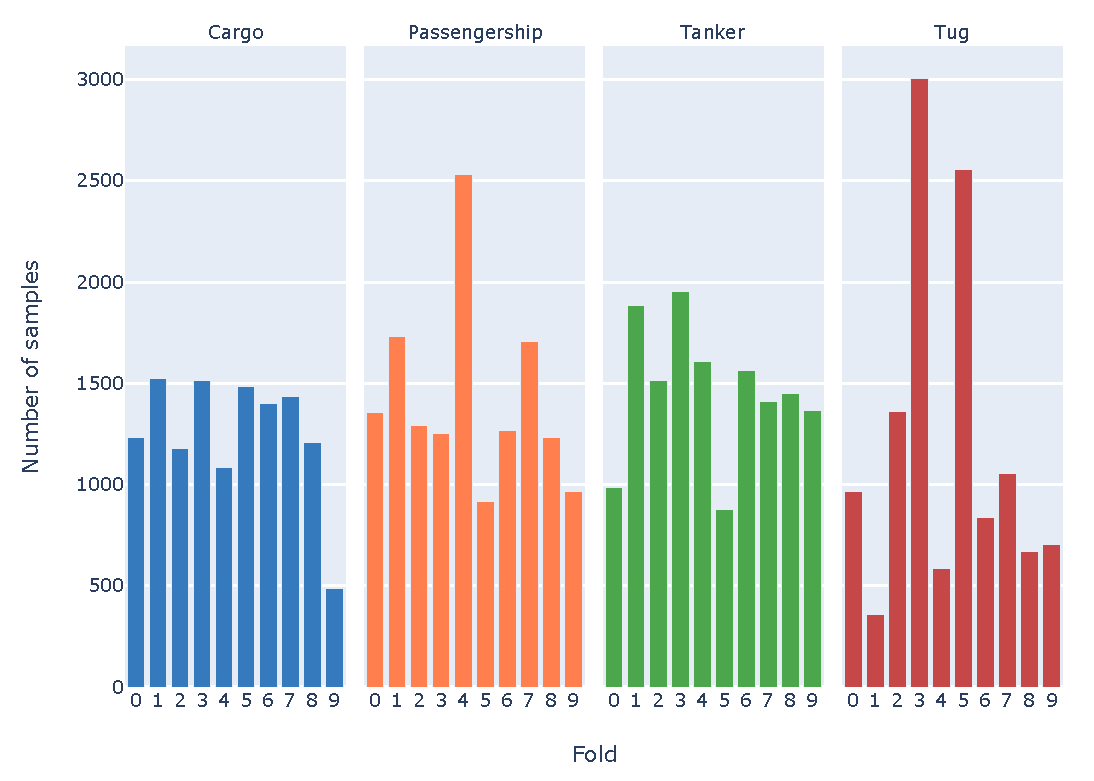
\includegraphics[width=0.95\textwidth]{img/ch3/10_fold_counts_facet.pdf}
        \caption{Count of samples in each class by fold}
        \label{fig:10-fold-counts-facet}
    \end{subfigure}
    \vfill
\end{figure}
\begin{figure}
    \ContinuedFloat
    % Subfigure 3: Spread of samples per class
    \begin{subfigure}[t]{\textwidth}
        \centering
        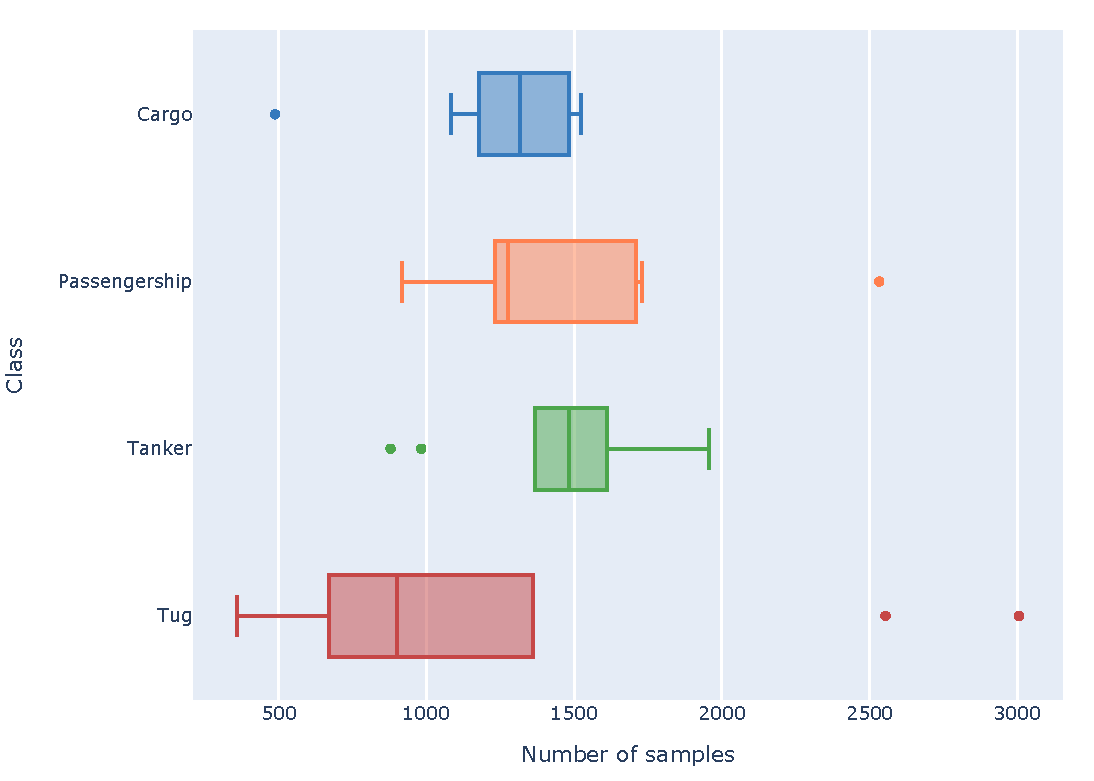
\includegraphics[width=0.95\textwidth]{img/ch3/10_fold_spread.pdf}
        \caption{Spread of samples in each fold by class}
        \label{fig:10-fold-spread}
    \end{subfigure}
    \caption{Distribution of samples across 10-fold split.}
    \label{fig:10-fold-overview}
\end{figure}

\subsection{Other standardised approaches}

Given the significant variation in segmentation and splitting methodologies across studies, as highlighted by Niu et al. \cite{niu_advances_2023}, there has been a recent trend towards adopting standardised train-test splits to enable more direct comparisons between classification techniques. In 2023, Zhu et al. proposed a specific division of the DeepShip dataset into 3-second segments for a consistent training and testing split \cite{zhu_underwater_2023}. This standardised split was published online \cite{zhupengsen_zhupengsenmethod-for-splitting--deepship-dataset_2024}, and several subsequent studies have since adopted this methodology to ensure comparability across research \cite{xu_self-supervised_2023, xu_self-supervised_2024, zhu_sfc-sup_2023, lin_underwater_2024}.

Zhu et al. also introduced a standardised background noise class to complement the DeepShip dataset. Unlike other datasets such as QiandaoEar22 (see Section \ref{subsubsec:qiandaoear22}), DeepShip lacks a dedicated background noise class due to the high level of shipping activity in the recording area, which means all recordings contain some degree of ship noise \cite{irfan_deepship_2021}. Although the original authors of DeepShip used over seven hours of external background noise recordings in their classifier, they did not disclose or publish these files. To address this, Zhu et al. provided a set of background noise files for future studies.

However, the inclusion of external background noise remains a point of debate. Some researchers, such as Tian et al., have incorporated background noise to improve classification performance \cite{tian_joint_2023}. However, others argue that this approach may not accurately reflect the specific acoustic environment of the DeepShip recordings.

For this study, we adhered to our own splitting methodology, consistent with the practices of Thales researchers, to maintain continuity across our internal projects. Furthermore, we opted not to augment the dataset with random noise samples, as we do not consider this step necessary or appropriate for accurately reflecting the operational environment represented in DeepShip.

%%%%%%%%%%%%%%%%%%%%%%%%%%%%%%%%%%%%%%%
\section{The classifier: CNN-LSTM}

The chosen classifier for the baseline model is CNN-LSTM, which aims to leverage the strengths of both \acrshort{cnn}s for spatial feature extraction and \acrshort{lstm} networks for sequential data processing. \acrshort{cnn}s excel at analysing spatial data, such as spectrograms of audio signals, while \acrshort{lstm}s are effective at modeling time-series data, identifying temporal patterns across sequences. By integrating CNN and \acrshort{lstm}, the hybrid architecture can capture both spatial and temporal features, making it well-suited for tasks such as time-series forecasting \cite{kim_predicting_2019, lu_cnn-lstm-based_2020}, natural language processing \cite{wang_dimensional_2016, umer_fake_2020}, and (as in our case) image classification in complex domains \cite{vankdothu_brain_2022, islam_combined_2020}. 

In the context of \acrshort{uatr}, this architecture serves as an ideal benchmark due to the spatial and temporal nature of sonar signal data. \acrshort{cnn}s can extract meaningful spatial features from spectrograms, while \acrshort{lstm}s sequentially process these extracted features, capturing unique temporal patterns that vary across vessel types due to differences in machinery, propulsion, and operating speeds. Thus, we believe that the CNN-LSTM classifier is well-positioned to benchmark the DeepShip dataset. 

\begin{sidewaysfigure}
    \centering
    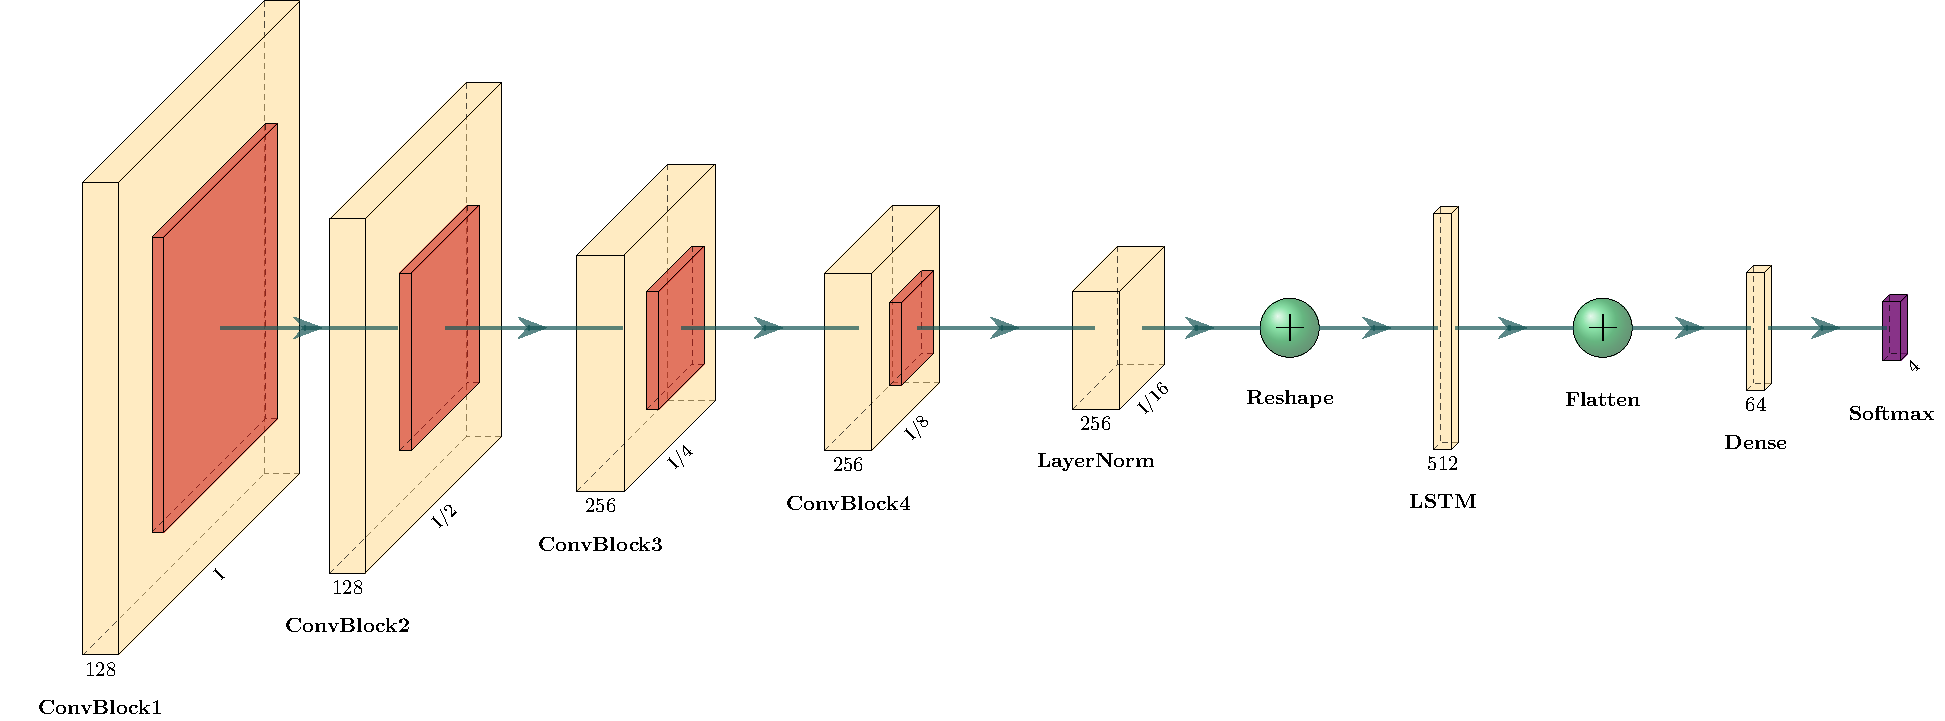
\includegraphics[width=\linewidth]{img/ch3/architecture_diagram.pdf}
    \caption{Baseline CNN-LSTM architecture diagram, illustrating key layers and their configurations. Each ConvBlock includes batch normalisation and ReLU activation, though these are not explicitly shown.}
    \label{fig:cnn-lstm-architecture}
\end{sidewaysfigure}

\subsection{Architecture layout}

The architecture starts with four convolutional blocks, each contributing to progressively deeper feature extraction, followed by an \acrshort{lstm} layer for temporal pattern recognition, and concluding with dense layers for final classification. A summary of each component is given below, and a diagram of the network can be found in Figure \ref{fig:cnn-lstm-architecture}.

\paragraph{Convolutional blocks 1 and 2} The first convolutional block applies a 2D convolution layer with 128 filters and a $5\times5$ kernel size, using padding to maintain spatial dimensions. The convolutional layer is followed by batch normalisation, which accelerates training and stabilises the learning process. A ReLU activation function introduces non-linearity, and a $2\times2$ max-pooling layer with a stride of $(2,2)$ down-samples the feature map, reducing spatial dimensions while retaining essential features. The second convolutional block is identical to the first, however, here the max-pooling size is increased to $(4,2)$ to further condense the feature representation.

\paragraph{Convolutional blocks 3 and 4} The third and fourth convolutional blocks replicate the structure of the first two blocks but with double the number of filters to enable the capture of more complex feature hierarchies. Both blocks use a $5\times5$ kernel, batch normalisation, ReLU activation, and max-pooling layers; however, in the final block, the max-pooling layer again uses a larger pooling window $(4, 2)$ to further down-sample the feature map, preparing it for sequential processing.

\paragraph{LSTM layer} After the convolutional blocks, the model incorporates a layer normalisation step to standardise the data. The output is then reshaped before being passed into the \acrshort{lstm} layer with 512 hidden units. The \acrshort{lstm} layer uses the hyperbolic tangent (tanh) as its activation function. This choice is based on TensorFlow's optimisation capabilities; when tanh is used as the activation function, TensorFlow can use an efficient cuDNN implementation on compatible GPUs, accelerating \acrshort{lstm} computations and maximising performance.

\paragraph{Classification layers} Following the \acrshort{lstm} layer, the output is flattened and passed through two fully connected (Dense) layers. The first dense layer, with 64 units and a ReLU activation, reduces the dimensionality and enables more complex learned representations, while the final dense layer, with 4 units and a softmax activation, outputs the class probabilities for the four vessel types under consideration.

\subsection{Input features}

The input feature chosen for our benchmark model was the power spectrogram. Power spectrograms apply a logarithmic transformation to the conventional spectrogram, calculated as $10 \cdot \log_{10}(P + \epsilon)$, representing the power or magnitude of the signal at each frequency over time. This logarithmic scaling brings the power spectrogram more in line with human auditory perception and also emphasises subtler sound components, making it both more visually interpretable and informative for analysis. The decision to use power spectrograms is well-supported by existing literature in underwater acoustics. For instance, previous studies, such as Cao et al. \cite{cao_underwater_2019}, have demonstrated the use of power spectrograms for extracting unique frequency features associated with vessel machinery, like shaft frequencies. 

To prepare the audio data for processing, each audio clip was first downsampled from its original rate of 32 kHz to 5 kHz. This choice was based on existing research such as papers by Arveson and Vendittis \cite{arveson_radiated_2000}, Malinowski et al. \cite{malinowski_underwater_2001}, Pricop et al. \cite{pricop_underwater_2010}, and McKenna et al. \cite{mckenna_underwater_2012}, which suggest that the 0-2 kHz frequency range captures the majority of relevant acoustic information for modern commercial ships. Hence, in-line with the Nyquist-Shannon sampling theorem, 5 kHz was chosen to maintain the most important frequency features whilst also reducing computational complexity. 

Each audio clip then underwent 0-1 normalisation to standardise amplitude levels across samples. This step aimed to mitigate the effects of loudness variations, allowing the machine learning model to focus on frequency-based characteristics rather than amplitude fluctuations.

The power spectrogram was then computed in MATLAB using the \texttt{spectrogram} function with the parameters listed in Table \ref{tab:powerspectrogram-parameters}. These parameters were selected to achieve a balanced trade-off between time and frequency resolution, suitable for capturing the distinctive spectral characteristics of different vessel types. The resulting power spectrograms initially had dimensions of 257 frequency bins $\times$ 116 time bins.

\begin{table}[htbp]
    \centering
    \begin{tabular}{ll}
        \toprule
        \textbf{Parameter}   & \textbf{Value} \\ \midrule
        Window length (\texttt{window}) & Hamming window of 256 samples \\
        Overlap (\texttt{noverlap})     & 128 samples (50\% overlap) \\
        FFT length (\texttt{nfft})      & 512 points  \\
        Sampling frequency (\texttt{fs}) & 5 kHz  \\ \bottomrule
    \end{tabular}
    \caption{STFT parameters for power spectrogram computation.}
    \label{tab:powerspectrogram-parameters}
\end{table}

Two additional preprocessing steps were applied to the power spectrogram matrices to optimise \acrshort{snr} and computational efficiency:
\begin{enumerate}
    \item DC offset removal: The extremely low-frequency components near 0 Hz were ignored as part of DC offset removal. Low-frequency components in underwater signals often contain high amplitudes due to constant offsets, which can introduce noise and large amplitude variations without providing useful classification information. By ignoring these low-frequency components, the power spectrogram better highlights informative portions of the spectrum, thus improving SNR.

    \item High-frequency cutoff: Based on an analysis of the frequency spectra of each vessel type, a high-frequency cutoff at 1000 Hz was applied. Figure \ref{fig:freq-ampl-highf} shows that for all vessel types analysed (Tug, Cargo, Passengership, and Tanker), significant energy is concentrated below 500 Hz, with a marked decline in amplitude beyond 1000 Hz. By 1500-2000 Hz, the amplitude is nearly negligible, suggesting minimal useful information at these higher frequencies. Setting the cutoff at 1000 Hz allows us to retain the most relevant frequency content while reducing the dimensionality and potential noise in the power spectrogram \cite{premus_machine_2020}. After applying the cutoff, the final power spectrogram matrices had dimensions of 100 frequency bins $\times$ 116 time bins.
\end{enumerate}
The final power spectrogram diagrams which were used as input to the machine learning model are shown in Figure \ref{fig:powerspectrogram-example}.

\begin{figure}[p]
    \centering
    \begin{subfigure}{0.49\textwidth}
        \centering
        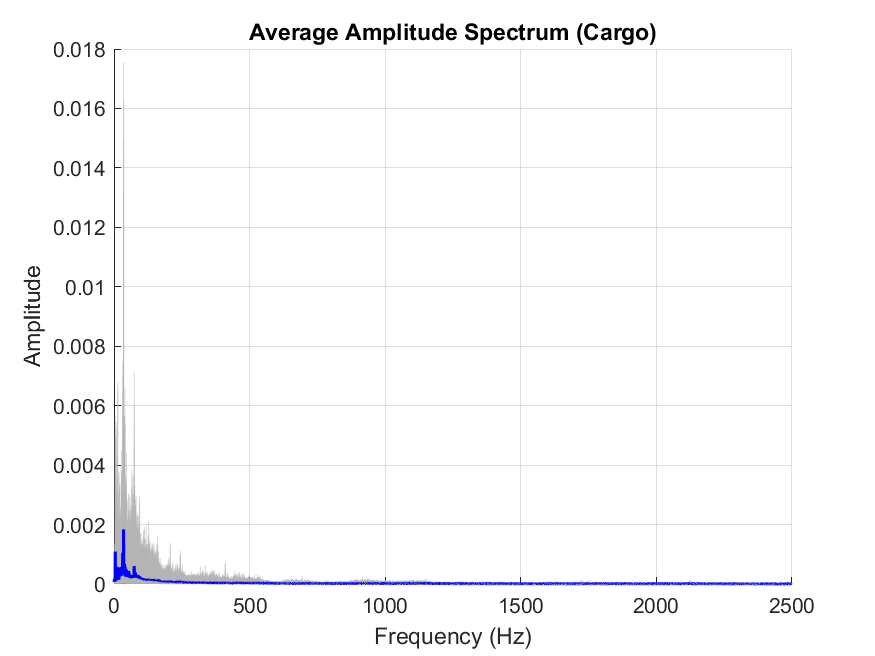
\includegraphics[width=\linewidth]{img/ch3/freq_ampl/cargo_freq_amplitude.png} 
    \end{subfigure}
    \hfill
    \begin{subfigure}{0.49\textwidth}
        \centering
        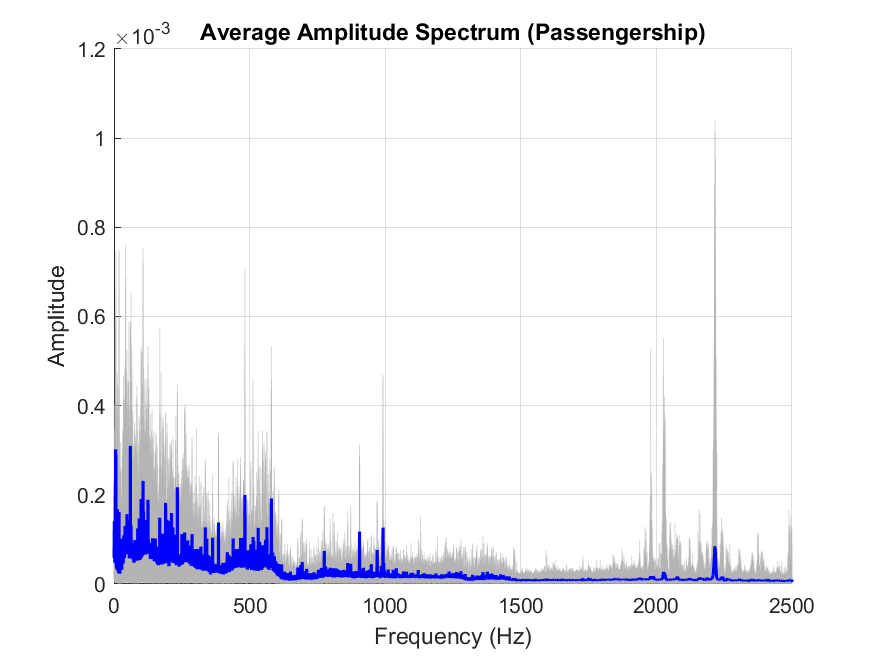
\includegraphics[width=\linewidth]{img/ch3/freq_ampl/passengership_freq_amplitude.png} 
    \end{subfigure}

    \vspace{0.5cm} % Space between rows

    \begin{subfigure}{0.49\textwidth}
        \centering
        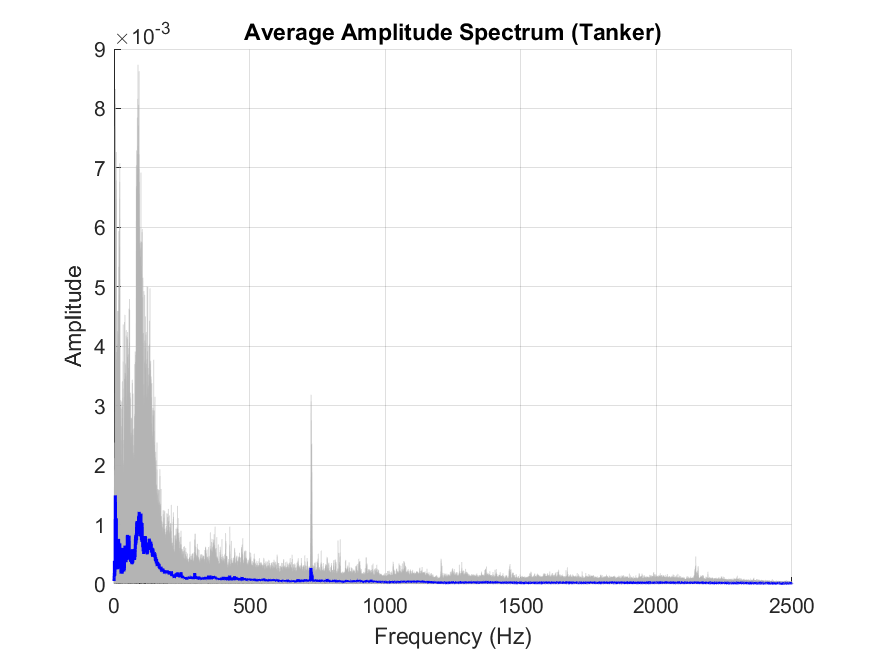
\includegraphics[width=\linewidth]{img/ch3/freq_ampl/tanker_freq_amplitude.png} 
    \end{subfigure}
    \hfill
    \begin{subfigure}{0.49\textwidth}
        \centering
        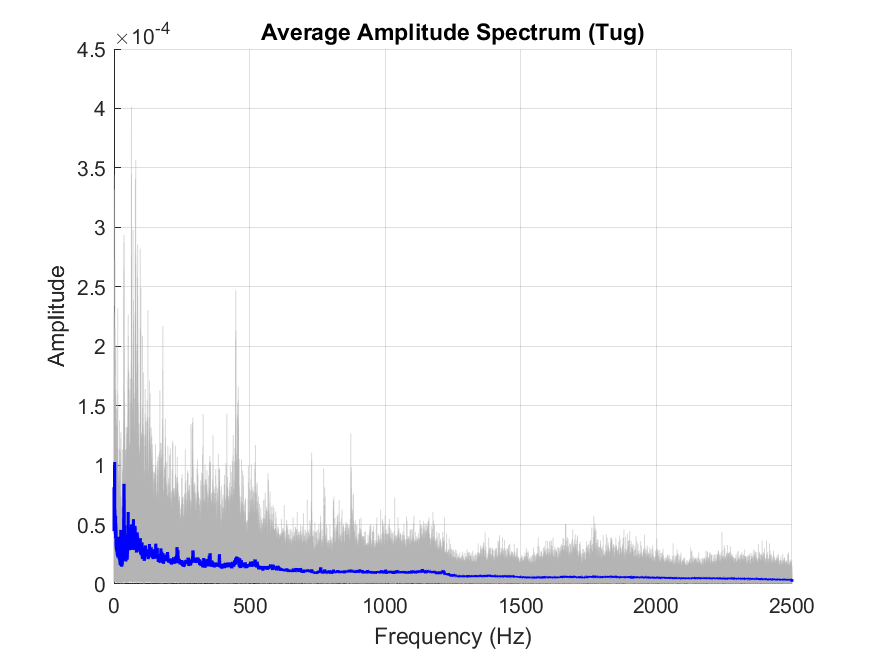
\includegraphics[width=\linewidth]{img/ch3/freq_ampl/tug_freq_amplitude.png} 
    \end{subfigure}

    \caption{Average single-sided amplitude spectra of each class. Faint gray lines represent individual segments, while the bold blue line indicates the average amplitude spectrum for each vessel type averaged over 100 segments.}
    \label{fig:freq-ampl-highf}
\end{figure}

\begin{figure}[p]
    \centering
    \begin{subfigure}{0.49\textwidth}
        \centering
        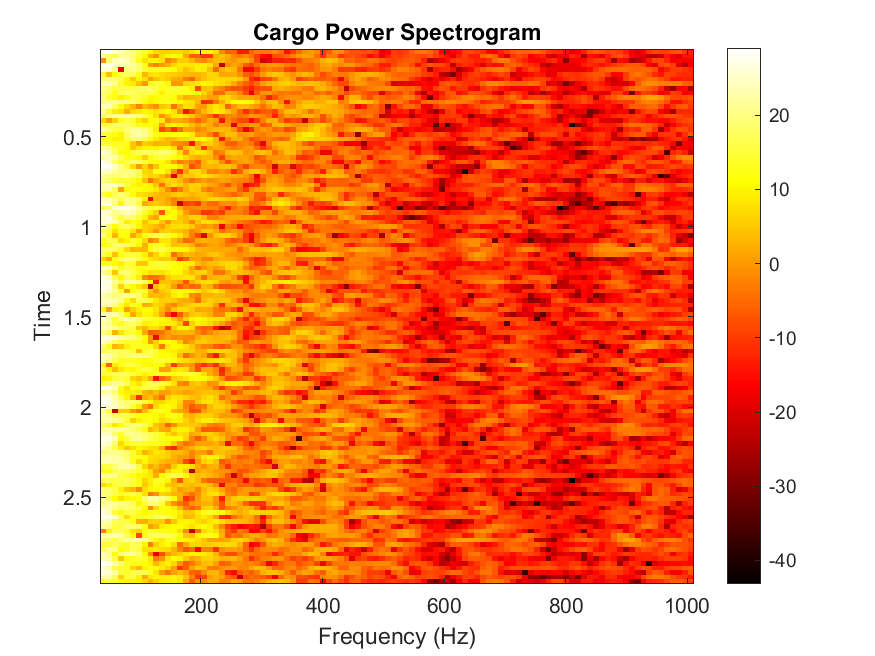
\includegraphics[width=\linewidth]{img/ch3/power_spectrogram/Cargo.png} 
    \end{subfigure}
    \hfill
    \begin{subfigure}{0.49\textwidth}
        \centering
        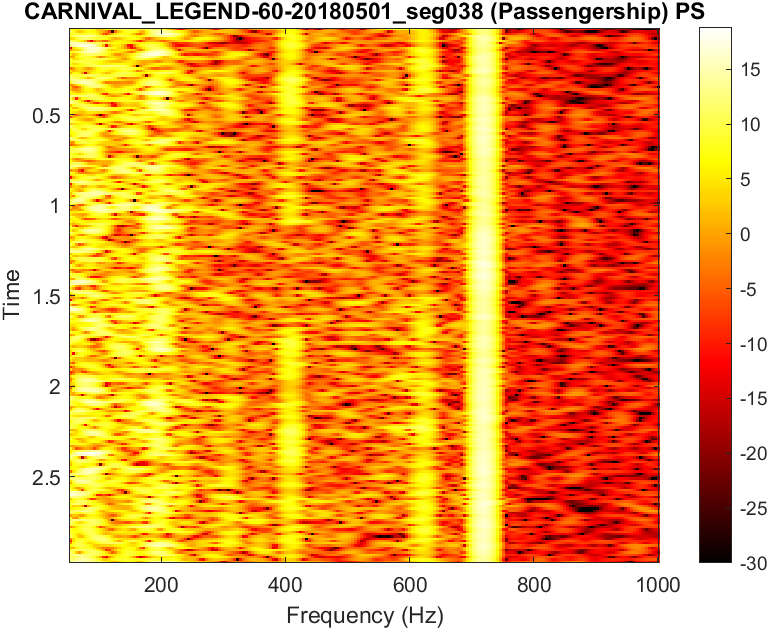
\includegraphics[width=\linewidth]{img/ch3/power_spectrogram/Passengership.png} 
    \end{subfigure}

    \vspace{0.5cm} % Space between rows

    \begin{subfigure}{0.49\textwidth}
        \centering
        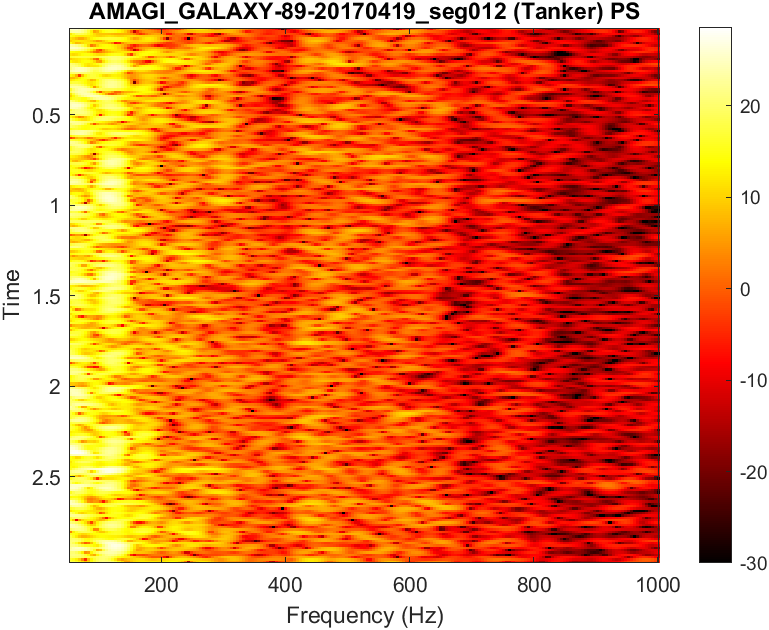
\includegraphics[width=\linewidth]{img/ch3/power_spectrogram/Tanker.png} 
    \end{subfigure}
    \hfill
    \begin{subfigure}{0.49\textwidth}
        \centering
        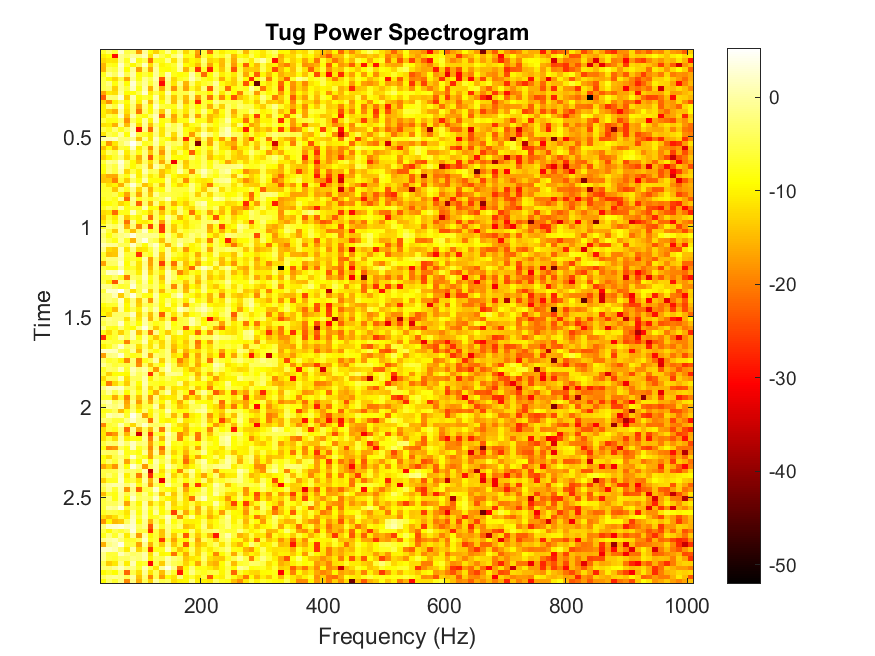
\includegraphics[width=\linewidth]{img/ch3/power_spectrogram/Tug.png} 
    \end{subfigure}
    \caption{Power spectrogram representations for each vessel class in the DeepShip dataset.}
    \label{fig:powerspectrogram-example}
\end{figure}


To facilitate efficient data loading in Python for model training, the power spectrograms were initially exported as CSV files and subsequently converted to compressed NumPy \texttt{npz} format. This conversion significantly improved I/O performance, enabling faster access to the data during model training. Finally, the data was organised into 10 data frames corresponding to the folds defined in the cross-validation setup.

\subsection{Training configuration}

For training, we used a combination of a batch size of 8, the Adam optimiser \cite{kingma_adam_2014}, and categorical cross-entropy as the loss function. We set the learning rate to $1 \times 10^{-5}$. %The Adam optimiser was chosen for its adaptive learning rate capabilities, which allow for dynamic adjustments during training.  
Training was set for 10 epochs using 20\% of the training data as a validation set to monitor performance. To prevent overfitting, we employed an early stopping callback that monitored the validation loss and halted training if no improvement was observed over 3 consecutive epochs. This callback also restored the model weights to the best-performing state recorded during training, ensuring optimal generalisation on the validation set.

As previously explained, to ensure a robust evaluation of the classifier's performance, we employed a 10-fold leave-one-out cross-validation approach. Practically, this meant that each iteration, nine folds were used for training and one fold was used for testing. This process was repeated 10 times, with each fold serving as the testing set once. The accuracy and loss were averaged across all 10 folds to provide a reliable estimate of the model's performance. This method helps mitigate the potential for overfitting to any specific subset of the data and provides a more comprehensive measure of the classifier's generalisation ability. A summary of the final training parameters can be found in Table \ref{tab:cnn-lstm-final-params}. 

All training was conducted on a Windows machine equipped with a NVIDIA GeForce RTX 2080 GPU (8GB) and 64GB of RAM, which provided sufficient computational resources for handling the dataset and training iterations. The baseline model was implemented using TensorFlow Keras (v2.10.0), and trained with CUDA (version 12.6), cuDNN (version 8.1.0), and cudatoolkit (version 11.2) libraries which are necessary for accelerated deep learning on NVIDIA GPUs. MATLAB processing was conducted using MATLAB version 2024a.

\begin{table}[htb]
\centering
\begin{tabular}{ll}
\toprule
\textbf{Parameter} & \textbf{Final value} \\ \midrule
Batch size & 8 \\
Optimiser & Adam \\
Loss function & Categorical cross-entropy \\
Learning rate & $1 \times 10^{-5}$ \\
Training epochs & 10 \\
Validation approach & Leave-one-out 10-fold cross validation \\
Callbacks & Early stopping (patience = 3 epochs) \\
Evaluation metrics & Accuracy, F1-score \\ \bottomrule
\end{tabular}
\caption{Final training parameters for benchmark CNN-LSTM model.}
\label{tab:cnn-lstm-final-params}
\end{table}

\subsection{Hyperparameter tuning}

The final architecture and training configuration described in the preceding sections were determined through an iterative process of hyperparameter tuning. Initially, the model architecture was designed with parameters based on standard practices for \acrshort{cnn}s and \acrshort{lstm} layers for time-series and spectral data. Specifically, the CNN layers used a filter size of $3 \times 3$ with 64 filters, while the \acrshort{lstm} layer included 1024 hidden units. The learning rate for training was set at $1 \times 10^{-3}$. However, we employed the Keras Tuner library to try and enhance our architecture and configuration. 

We used Keras Tuner's \texttt{RandomSearch} method for hyperparameter tuning. Random search is particularly well-suited for projects with large search spaces and limited computation resources, as alternative methods (such as Bayesian optimisation) often require the direct modelling of dependencies between parameters -- a computationally expensive step. Using random search allowed us to find the most promising configurations in a relatively short time.

The hyperparameters included in the search space, as well as a brief motivation for tuning each of them, is provided below. 

\begin{itemize} 
\item \textbf{Number of filters and filter size}: We tested kernel sizes of length $[3, 5, 7]$ to evaluate how receptive field size affects the model's ability to capture spatial features. We also varied the number of filters in each convolutional layer across $[32, 64, 128, 256]$.
\item \textbf{LSTM units}: We tested \acrshort{lstm} configurations with 
$[256, 512, 1024, 2048]$ units to determine the optimal memory capacity for capturing temporal dependencies. 
\item \textbf{Dense layer units and activation function}: For the dense layer immediately after \acrshort{lstm}, we experimented with $[32, 64, 128, 256]$ units and evaluated both \texttt{relu} and \texttt{tanh} activations to observe which non-linearity best captures high-level abstractions in the data. 
\item \textbf{Optimiser}: The choice of optimiser can significantly impact convergence; we compared \texttt{adam}, \texttt{rmsprop}, and \texttt{sgd}. 
\item \textbf{Learning rate}: Four different learning rates were tested to find the best balance between learning speed and stability: $1 \times 10^{-5}$, $1 \times 10^{-4}$, $1 \times 10^{-3}$ and $1 \times 10^{-2}$.
\end{itemize}

A summary of the search space alongside the hyperparameter configuration yielding the best performance is provided in Table \ref{tab:hyperparameter-search-space}.

\begin{table}[htbp] 
\centering 
    \begin{tabular}{lll} 
    \toprule 
    \textbf{Hyperparameter} & \textbf{Values tested} & \textbf{Optimal value} \\ 
    \midrule 
    Filter size (\texttt{filter\_size}) & 3, 5, 7 & 5 \\ 
    Number of filters (\texttt{num\_filters}) & 32, 64, 128, 256 & 128 \\ 
    LSTM units (\texttt{lstm\_units}) & 256, 512, 1024, 2048 & 512 \\ 
    Dense layer units (\texttt{dense\_units}) & 32, 64, 128, 256 & 64 \\ 
    Dense layer activation (\texttt{dense\_activation}) & \texttt{relu}, \texttt{tanh} & \texttt{relu} \\ 
    Optimiser (\texttt{optimizer}) & \texttt{adam}, \texttt{rmsprop}, \texttt{sgd} & \texttt{adam} \\ 
    Learning rate (\texttt{learning\_rate}) & 1e-5, 1e-4, 1e-3, 1e-2 & $1 \times 10^{-5}$ \\ 
    \bottomrule 
    \end{tabular} 
\caption{Hyperparameter search space used for model tuning with ideal configuration.} 
\label{tab:hyperparameter-search-space} 
\end{table}

These results highlight that a larger filter size and an increased number of filters in the \acrshort{cnn} layers improved the model's feature extraction capability, while a reduction in \acrshort{lstm} units (from the initial 1024 to 512) helped balance memory capacity with computational efficiency. Additionally, a low learning rate of $1 \times 10^{-5}$ with the Adam optimiser yielded the best results, likely due to its ability to maintain stable updates in high-dimensional spaces.

Based on these results, the final network architecture was modified to incorporate the optimal hyperparameters. The \acrshort{cnn} was configured with a $5\times5$ filter size and 128 filters, while the \acrshort{lstm} layer used 512 hidden units. The dense layer was set to 64 units with \texttt{relu} activation. Training was carried out with the Adam optimiser and a learning rate of $1 \times 10^{-5}$. This process of hyperparameter tuning not only improved the model's performance but also provided insights into the configuration choices that best capture the temporal and spectral features for \acrlong{uatr}.

\subsection{Final benchmark results}

After training the benchmark CNN-LSTM model with the final parameters detailed in Table \ref{tab:cnn-lstm-final-params}, we achieved an \textbf{overall baseline accuracy of 86.67\%}. Additionally, the model demonstrated a strong average performance across key classification metrics: precision (87.29\%), recall (86.67\%), and F1 score (86.74\%).

The training and validation accuracy-loss curves for each fold, shown in Figure \ref{fig:cnn-lstm-acc-loss-training-plot}, illustrate the model's performance over the 10 epochs, with noticeable early-stopping in some folds based on the early-stopping callback applied to prevent overfitting. 

\begin{figure}[htbp]
    \centering
    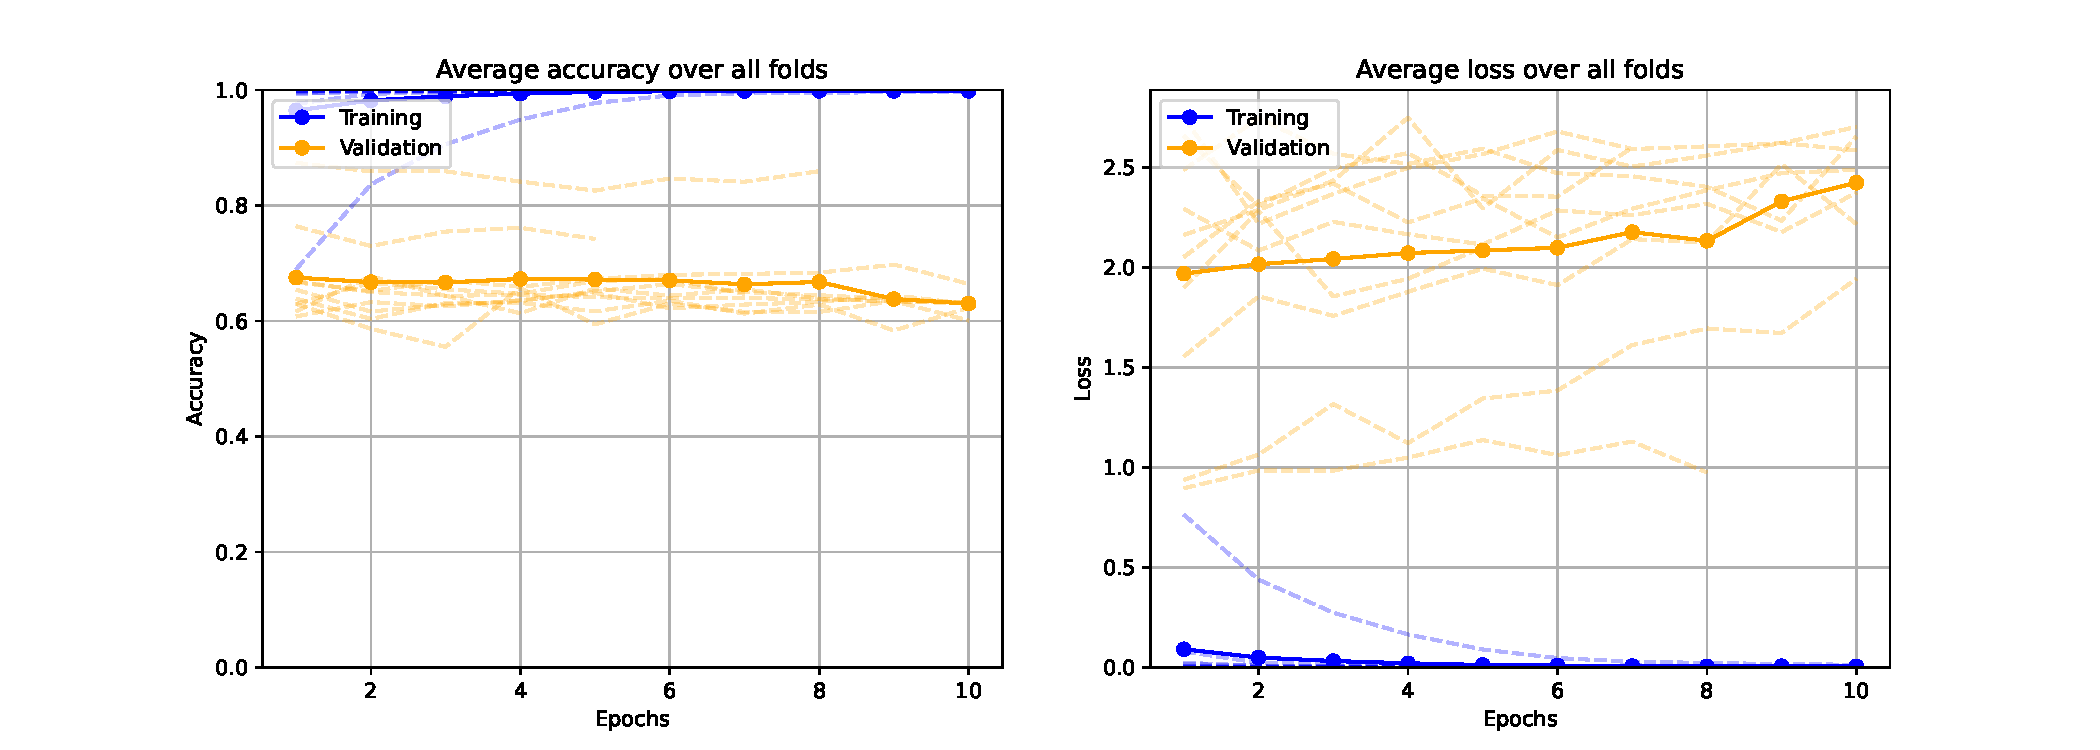
\includegraphics[trim={2cm 0 2cm 0},clip,width=\textwidth]{img/ch3/cnn_lstm_acc_loss.pdf}
    \caption{Average training and validation accuracy and loss over ten epochs for the benchmark CNN-LSTM model, with results averaged across all folds.}
    \label{fig:cnn-lstm-acc-loss-training-plot}
\end{figure}

These metrics collectively establish a robust benchmark for evaluating the effectiveness of different preprocessing and feature extraction techniques.